\chapter{PyLith Design}
\label{cha:design}

PyLith is separated into modules to encapsulate behavior and facilitate
use across multiple applications. This allows expert users to replace
functionality of a wide variety of components without recompiling
or polluting the main code. PyLith employs external packages (see
Figure \vref{fig:pylith:dependencies}) to reduce development time
and enhance computational efficiency; for example, PyLith 0.8 ran
two times faster when the PETSc linear solver was used.

\begin{figure}[htbp]
  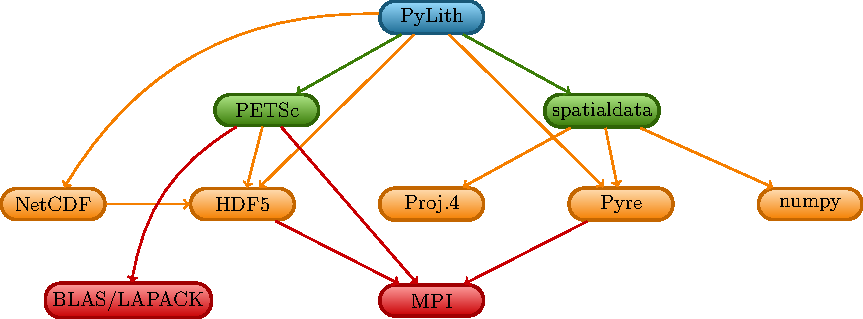
\includegraphics[width=4in]{implementation/figs/packages}
  \caption{PyLith dependencies. PyLith makes direct use of several
    other packages, some of which have their own dependencies.}
  \label{fig:pylith:dependencies}
\end{figure}

PyLith is written in two programming languages. High-level code is
written in Python; this rich, expressive interpreted language with
dynamic typing reduces development time and permits flexible addition
of user-contributed modules. This high-level code makes use of Pyre, a
science-neutral simulation framework developed at Caltech by Michael
Aivazis, to link the modules together at runtime and gather
user-input. Low-level code is written in C++, providing fast execution
while still allowing an object-oriented implementation. This low-level
code relies on PETSc for finite-element data structures, time-stepping
algorithms, and solvers. We use SWIG to create Python bindings for the
C++ objects.

In writing PyLith 1.0, the code was designed to be object-oriented and
modular. Each type of module is accessed through a specified interface
(set of functions). This permits adding, replacing, and rewriting
modules without affecting other parts of the code. This code structure
simplifies code maintenance and development. Extending the set of code
features is also easier, since developers can create new modules
derived from the existing ones.

The current code design leverages Pyre and PETSc extensively. Pyre
glues together the various modules used to construct a simulation and
specify the parameters. Most of the PyLith source code pertains to
implementing the geodynamics, such as the governing equations, bulk
rheology, boundary conditions, and earthquake rupture via slip on
faults.

Nemesis (Pyre subpackage) allows PyLith to run Python using the
Message Passing Interface (MPI) for parallel processing. Additional,
indirect dependencies (see Figure \vref{fig:pylith:dependencies})
include numpy (efficient operations on numerical arrays in Python),
Proj.4 (geographic projections).

During development we implement three levels of testing: (1) unit
testing, which occurs at the class/function level, (2) testing via the
Method of Manufactured Solutions to test the finite-element
implementation of the governing equations, and (3) full-scale testing,
which involves complete PyLith simulations. We run these tests
throughout the development cycle to expose bugs and isolate their
origin. As additional changes are made to the code, the tests are
rerun to help prevent introduction of new bugs.

Additionally, we use community benchmarks, such as developed through
the Southern California Earthquake Center for crustal deformation and
dynamic rupture to determine the relative local and global error (see
Chapter \vref{sec:benchmarks}).

\section{Pyre}

Pyre is an object-oriented environment capable of specifying and launching
numerical simulations on multiple platforms, including Beowulf-class
parallel computers and grid computing systems. Pyre allows the binding
of multiple components such as solid and fluid models used in Earth
science simulations, and different meshers. The Pyre framework enables
the elegant setup, modification and launching of massively parallel
solver applications.

\begin{figure}[htbp]
  \includegraphics[width=4in]{intro/figs/pyre_overview}
  \caption{Pyre Architecture. The integration framework is a set of
    cooperating abstract services.}
  \label{fig:Pyre:Architecture}
\end{figure}

Pyre is a framework, a combination of software and design philosophy
that promotes the reuse of code. In the context of frameworks and
object-oriented programming, Pyre can be thought of as a collection of
classes and the way their instances interact.  Programming
applications based on Pyre will look similar to those written in any
other object-oriented language. 

The Pyre framework incorporates features aimed at enabling the
scientific non-expert to perform tasks easily without hindering the
expert. Target features for end users allow complete and intuitive
simulation specification, reasonable defaults, consistency checks of
input, good diagnostics, easy access to remote facilities, and status
monitoring. Target features for developers include easy access to user
input, a shorter development cycle, and good debugging support.


\section{PETSc}

PyLith 2.x and later make use of a set of data structures and routines
in PETSc called \object{DMPlex}, which is still under active
development. \object{DMPlex} provides data structures and routines for
for representing and manipulating computational meshes, and it greatly
simplifies finite-element computations.\object{DMPlex} represents the
topology of the domain. Zero volume elements are inserted along all
fault surfaces to implement kinematic (prescribed) or dynamic
(constitutive model) implementations of fault slip. Material
properties and other parameters are represented as scalar and vector
fields over the mesh using vectors to store the values and sections to
map vertices, edges, faces, and cells to indices in the vector. For
each problem, functions are provided to calculate the residual and its
Jacobian.  All numerical integration is done in these functions, and
parallel assembly is accomplished using the get/set closure paradigm
of the \object{DMPlex} framework.

PETSc \url{www-unix.mcs.anl.gov/petsc/petsc-as}, the Portable,
Extensible Toolkit for Scientific computation, provides a suite of
routines for parallel, numerical solution of partial differential
equations for linear and nonlinear systems with large, sparse systems
of equations.  PETSc includes time-stepping algorithms and solvers
that implement a variety of Newton and Krylov subspace methods. It can
also interface with many external packages, including ESSL, MUMPS,
Matlab, ParMETIS, PVODE, and Hypre, thereby providing additional
solvers and interaction with other software packages.

PETSc includes interfaces for FORTRAN 77/90, C, C++, and Python for
nearly all of the routines, and PETSc can be installed on most Unix
systems. Users can use PETSc parallel matrices, vectors, and other
data structures for most parallel operations, eliminating the need for
explicit calls to Message Passing Interface (MPI) routines. Many
settings and options can be controlled with PETSc-specific
command-line arguments, including selection of preconditions, solvers,
and generation of performance logs.


\section{Finite-Element Implementation User Interface}

In specifying simulation parameters, some details of the
finite-element implementation using the PETSc \object{DMPlex} is
exposed to the user. In this section we describe the data structures
to give the user greater context for understanding what the parameters
mean.

\tip{See the dveloper guide in Chapter \vref{cha:developer} for a
  detailed discussion of the implementation and organization of the
  PyLith code.}

\subsection{Fields and Subfields}

Finite-element coefficients for the finite-element basis functions
(sometimes thought of as the values at vertices, on edges and faces,
or in cells) are stored in a \object{Field}. A \object{Field} is
composed of a \object{Section}, which associates the points (vertices,
edges, faces, and cells) with the finite-element coefficients, and a
\object{Vec}, which is a vector storing the finite-element
coefficients. A \object{Field} may hold a single subfield, such as
displacement, or it may hold several subfields, such as the density,
shear modulus, and bulk modulus for an isotropic, linear elastic
material.

Spatial discretization is specified for each subfield. That is, each subfield
within a \object{Field} can have a different discretization. For
example, a displacement field may use a second order discretization
while a pressure field may use a first order discretization. If we
have uniform material properties, we use a zero order discretization
(uniform values within a cell) to reduce the storage requirements.

The two main types of fields are the solution field and auxiliary
fields.

\subsubsection{Solution Field}

The solution field contains all of the finite-element coefficients
corresponding to the problem solution. As discussed in the
multiphysics finite-element formulation in
Section~\label{sec:multiphysics:formulation}, if the governing
equations have multiple unknowns, such as displacement and fluid
pressure for poroelasticity, then the solution field will have
multiple subfields.  See Section \vref{sec:solution:user:interface} for
details of the user interface and predefined containers for common
subfield collections.

\subsubsection{Auxiliary Field}

We specify parameters for materials, boundary conditions, and fault
interfaces using fields we refer to as the ``auxiliary'' fields.  Each
parameter (scalar, vector, tensor, or other) is held in a separate
subfield. We also store state variables in the auxiliary field, with
each state variable as a different subfield. This provides a single
container for the collection of spatially varying parameters while
maintaining the flexibility to specify the discretization of each
parameter separately. 

\subsubsection{Discretization}

The discretization of the field is given in terms of the topology
(vertices, edges, faces, and cells) associated with the field and the
basis order and quadrature order. The basis order refers to the
highest order in the basis functions. For example, a basis order of 0
has just a constant and a basis order of 2 for a polynomial basis has
constant, linear, and quadratic terms.

\warning{Currently, the quadrature order {\bf MUST} be the same for
  all subfields in a simulation. This restriction may be relaxed in
  the future. PyLith will check this and indicate if a subfield has a
  quadrature order that does not match the first solution subfield.}


% End of file
